% Options for packages loaded elsewhere
\PassOptionsToPackage{unicode}{hyperref}
\PassOptionsToPackage{hyphens}{url}
\documentclass[
  10pt,
]{article}
\usepackage{xcolor}
\usepackage[margin=20mm]{geometry}
\usepackage{amsmath,amssymb}
\setcounter{secnumdepth}{-\maxdimen} % remove section numbering
\usepackage{iftex}
\ifPDFTeX
  \usepackage[T1]{fontenc}
  \usepackage[utf8]{inputenc}
  \usepackage{textcomp} % provide euro and other symbols
\else % if luatex or xetex
  \usepackage{unicode-math} % this also loads fontspec
  \defaultfontfeatures{Scale=MatchLowercase}
  \defaultfontfeatures[\rmfamily]{Ligatures=TeX,Scale=1}
\fi
\usepackage{lmodern}
\ifPDFTeX\else
  % xetex/luatex font selection
  \setmainfont[]{Times New Roman}
\fi
% Use upquote if available, for straight quotes in verbatim environments
\IfFileExists{upquote.sty}{\usepackage{upquote}}{}
\IfFileExists{microtype.sty}{% use microtype if available
  \usepackage[]{microtype}
  \UseMicrotypeSet[protrusion]{basicmath} % disable protrusion for tt fonts
}{}
\makeatletter
\@ifundefined{KOMAClassName}{% if non-KOMA class
  \IfFileExists{parskip.sty}{%
    \usepackage{parskip}
  }{% else
    \setlength{\parindent}{0pt}
    \setlength{\parskip}{6pt plus 2pt minus 1pt}}
}{% if KOMA class
  \KOMAoptions{parskip=half}}
\makeatother
\setlength{\emergencystretch}{3em} % prevent overfull lines
\providecommand{\tightlist}{%
  \setlength{\itemsep}{0pt}\setlength{\parskip}{0pt}}
\usepackage{bookmark}
\IfFileExists{xurl.sty}{\usepackage{xurl}}{} % add URL line breaks if available
\urlstyle{same}
\hypersetup{
  hidelinks,
  pdfcreator={LaTeX via pandoc}}

\author{}
\date{}

\usepackage{graphicx}
\begin{document}

\section{Supplemental Material: resource, timing, and paired-effect
evidence}\label{supplemental-material-resource-timing-and-paired-effect-evidence}

This material supplements the code-capacity results in the manuscript.
The plots reuse the samples described in Sec. III A and therefore do not
constitute independent evaluations. The repository-local source index is
in \url{ARCHIVE_DATA_INDEX.md}. A public archive identifier and access
URL remain to be supplied before submission.

\subsection{S1. Accuracy versus search
resources}\label{s1.-accuracy-versus-search-resources}

\begin{center}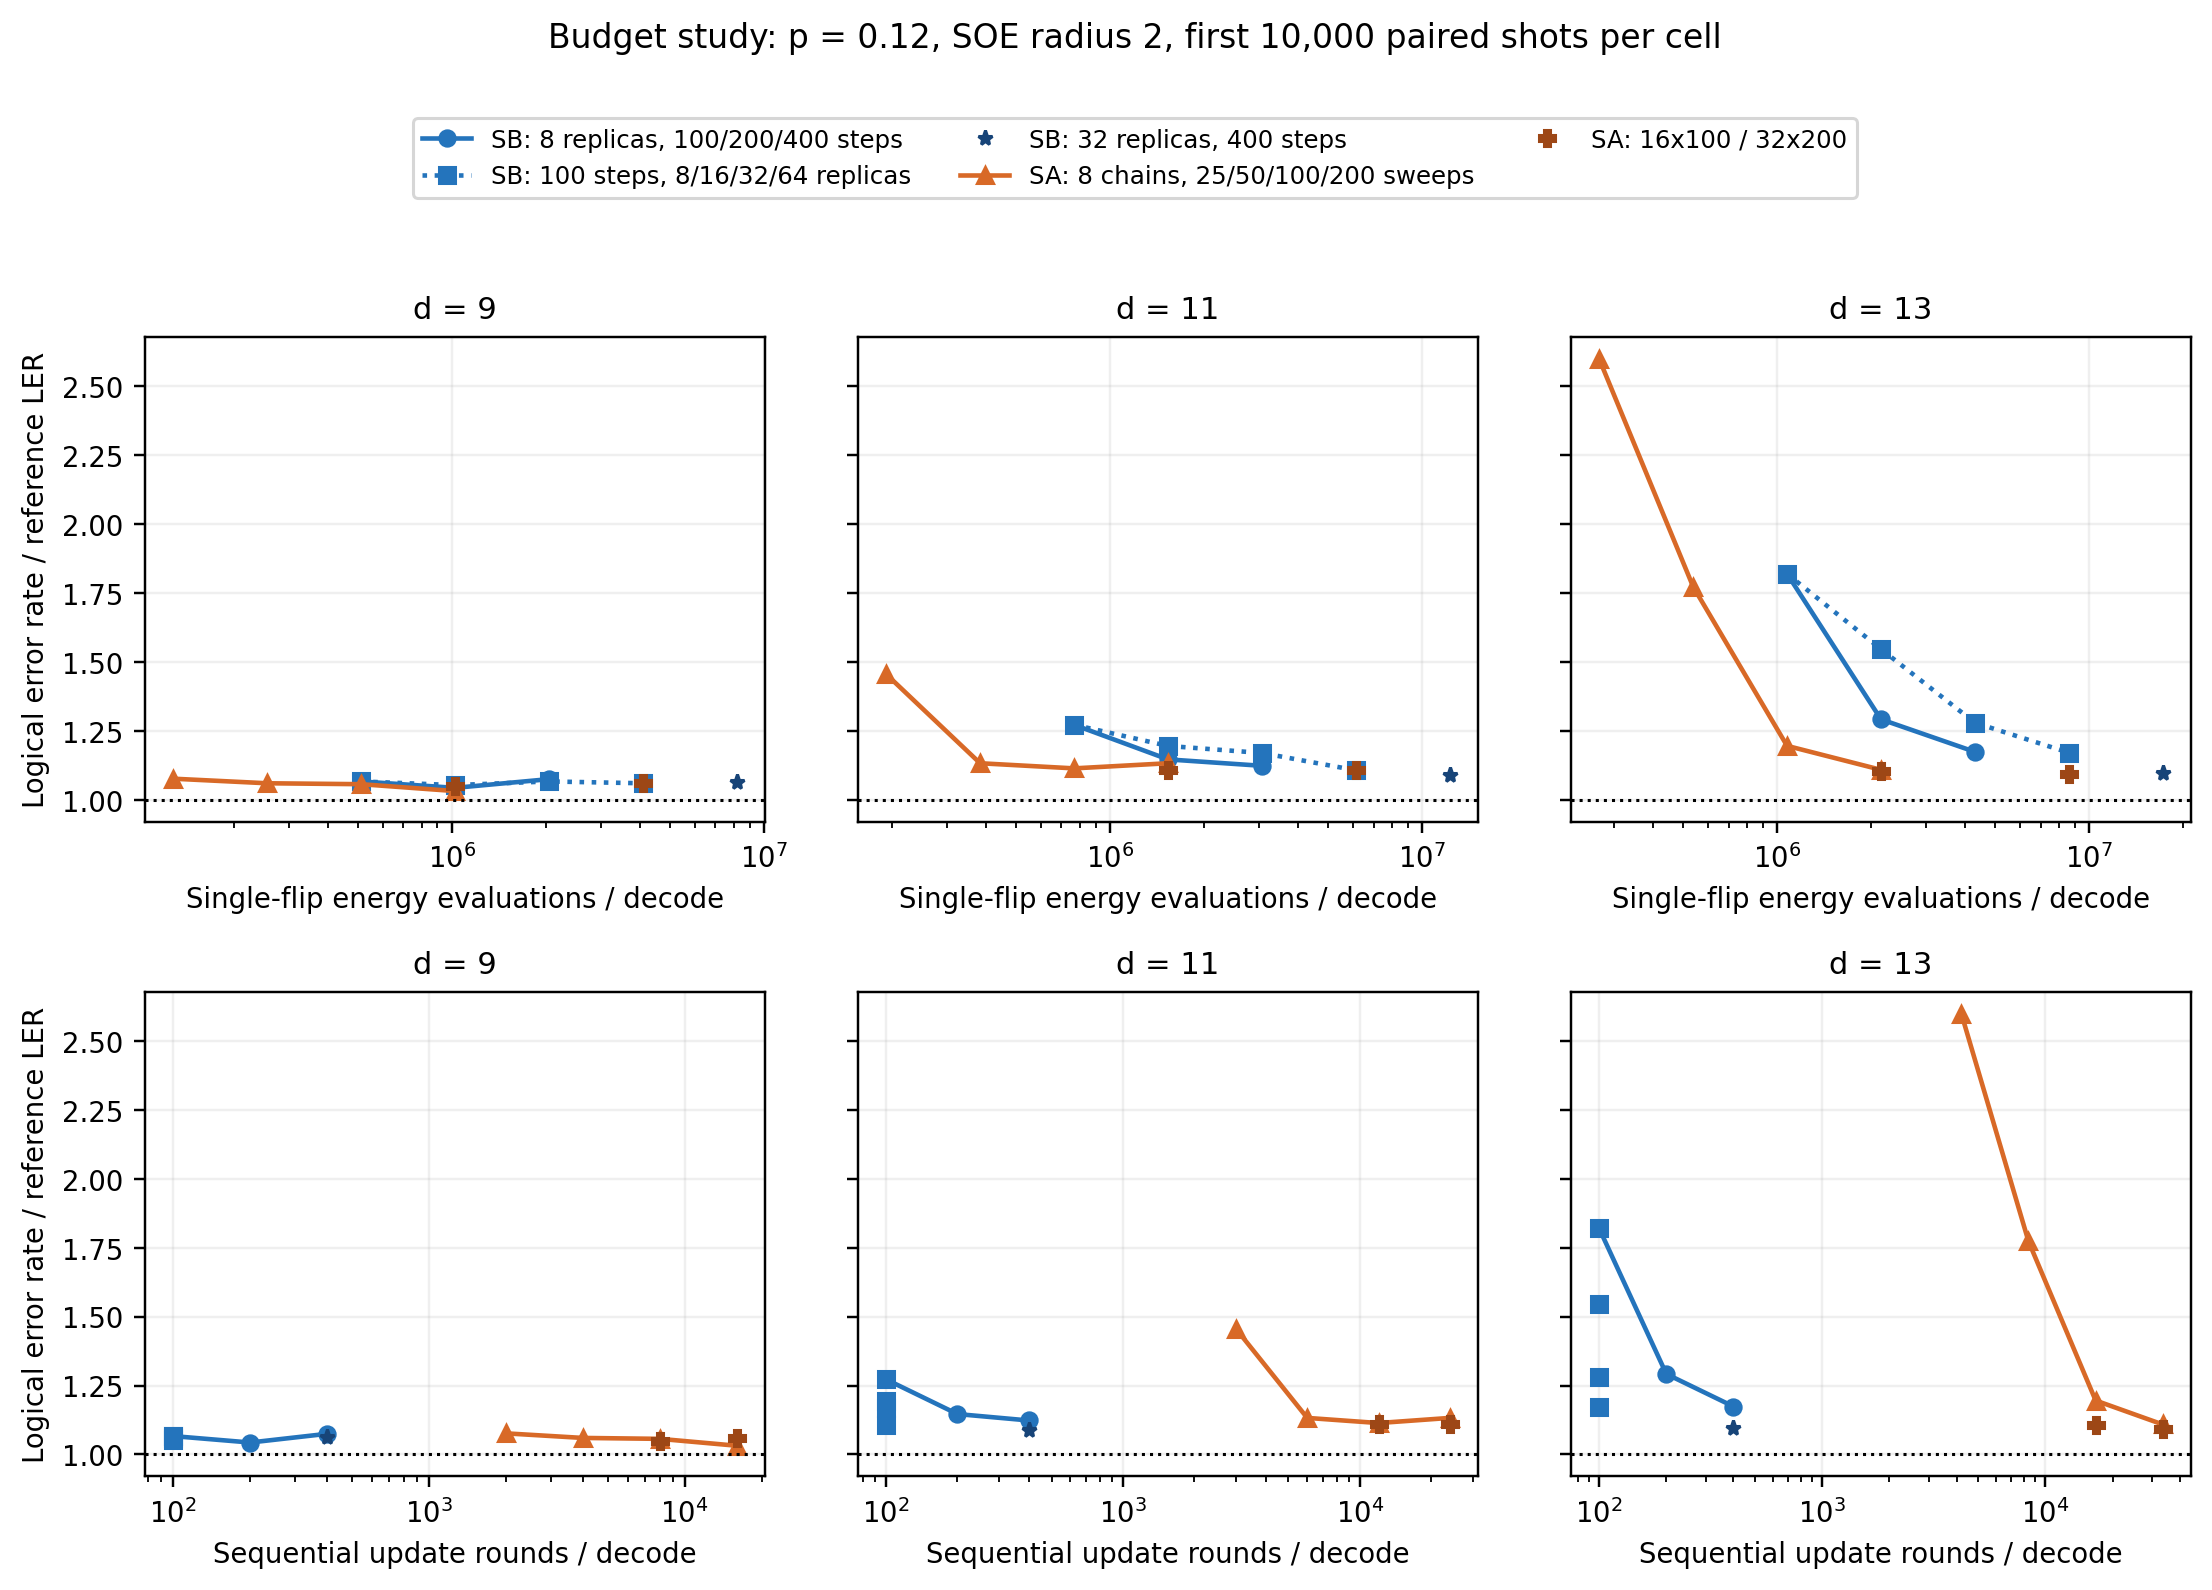
\includegraphics[width=\textwidth,height=0.55\textheight,keepaspectratio]{figures/resources_p0.12.png}\end{center}

\textbf{Figure S1. Accuracy versus two search resources at \(p=0.12\).}
Columns show \(d=9,11,13\). The upper row plots LER/REF against total
flip-energy evaluations; the lower row uses sequential update rounds.
Horizontal axes are logarithmic. Every point uses SOE radius two and the
same 10,000 shots within its cell. Blue circles increase SB steps at
eight replicas; blue squares increase replicas at 100 steps; the blue
star denotes \(32\times400\). Orange triangles increase SA sweeps at
eight chains, and additional SA budgets are marked separately. Both rows
use the same accuracy point estimates. Supplemental Fig. S2 gives paired
uncertainty for selected comparisons. The horizontal coordinates count
search work and sequential rounds under Eq. (10), not measured runtime
or complete end-to-end cost. Changing the replica count at a fixed
number of SB steps leaves the round count unchanged. Additional noise
slices are linked in the Supplemental Material; the \(p=0.18\) slice
contains only the configurations evaluated there.

For measured time, see the optimized CP accuracy--time comparison in
manuscript Figure 4; the resource counts above exclude complete
end-to-end costs.

\newpage

\subsection{S2. Paired effect sizes}\label{s2.-paired-effect-sizes}

\begin{center}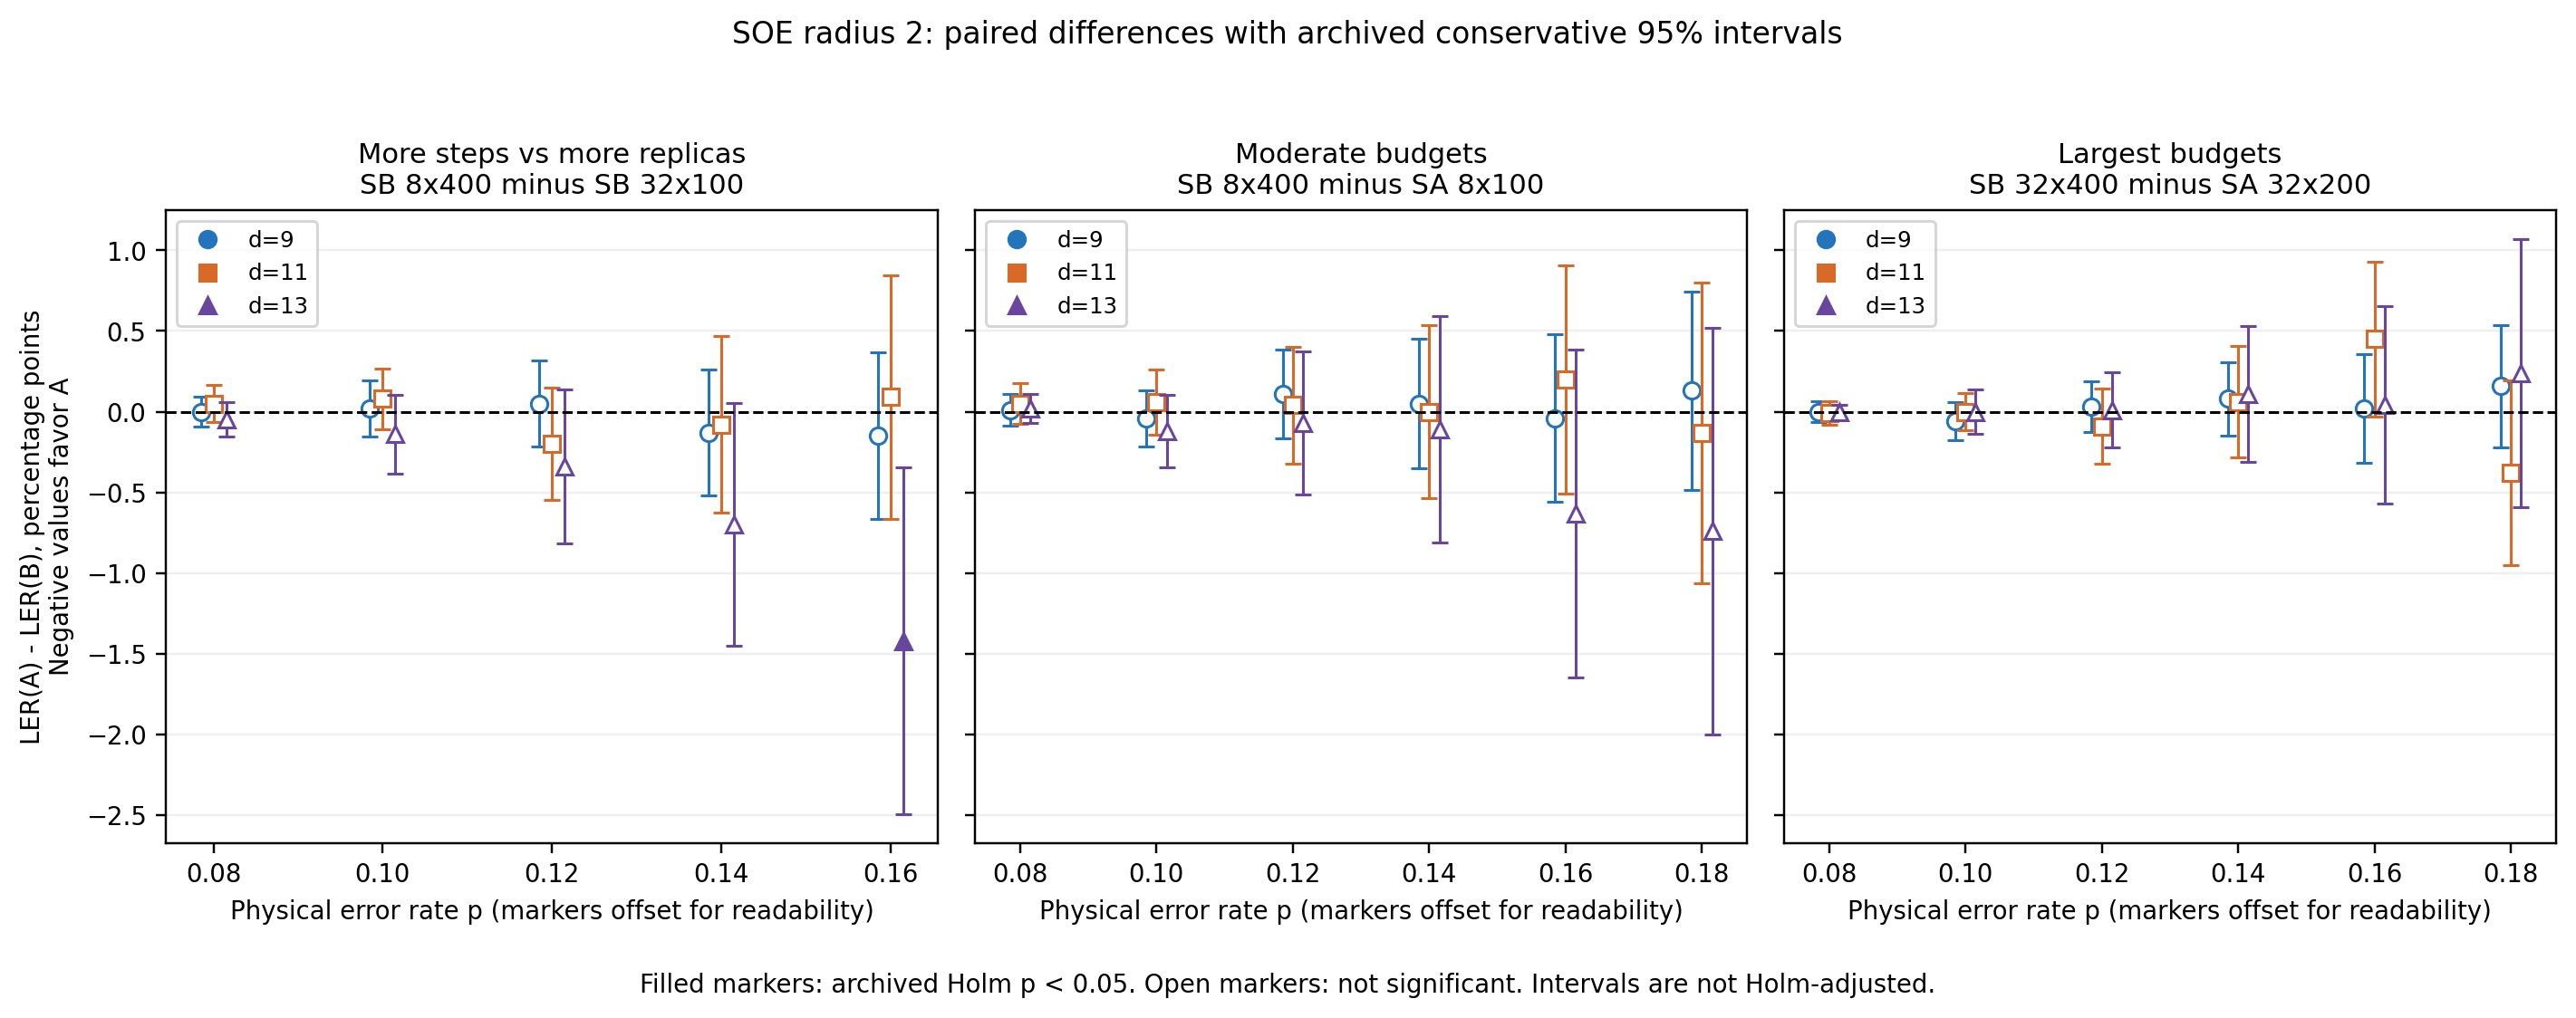
\includegraphics[width=\textwidth,height=0.55\textheight,keepaspectratio]{figures/paired_improvements_r2.png}\end{center}

\textbf{Figure S2. Paired effect sizes for budget comparisons.} The
horizontal axis is physical error probability; small marker offsets are
for display only. The vertical coordinate is
\(100[\mathrm{LER}(A)-\mathrm{LER}(B)]\), in percentage points; negative
values favor the first configuration named in each panel. Panels compare
SB \(8\times400\) with SB \(32\times100\), SB \(8\times400\) with SA
\(8\times100\), and SB \(32\times400\) with SA \(32\times200\). All use
radius two. Color and marker shape identify distance. Error bars are
conservative per-cell 95\% intervals obtained by differencing
Bonferroni-allocated Clopper--Pearson intervals for the two
discordant-outcome probabilities. They are not Holm-adjusted
simultaneous intervals across cells. Filled markers indicate an exact
paired test with an archived Holm-adjusted value below 0.05, using the
comparison families defined in Sec. III C; the tests are not
recalculated for the displayed subset. The intervals and corrected tests
are distinct procedures; absence of significance does not establish
equivalence. The left panel covers 15 cells at \(p=0.08\)--0.16; the
other panels cover 18 cells at \(p=0.08\)--0.18. SB \(32\times100\) was
not evaluated at \(p=0.18\).

The intervals and Holm-adjusted tests answer different statistical
questions. Neither nonsignificance nor overlapping intervals establish
equivalence.

\subsection{S3. Additional resource
slices}\label{s3.-additional-resource-slices}

The following five pages contain the
\href{figures/resources_p0.08.pdf}{p = 0.08},
\href{figures/resources_p0.10.pdf}{0.10},
\href{figures/resources_p0.14.pdf}{0.14},
\href{figures/resources_p0.16.pdf}{0.16}, and
\href{figures/resources_p0.18.pdf}{0.18} slices, which use the same
resource definitions as Supplemental Fig. S1. The p = 0.18 slice
includes only configurations evaluated at that noise rate. These slices
provide additional views of the same observations.

\end{document}
